\documentclass{article}
\usepackage[margin=1.5cm]{geometry}
\usepackage{amsmath}
\usepackage{cases}
\usepackage{accents}
\usepackage{caption} 
\oddsidemargin = 13pt
\textwidth = 426pt
\marginparwidth = 65pt
\usepackage{graphicx}

\begin{document}
	\title{TIPE 2025 - Pendule de Foucault}
	\author{Julien ROPERS, May SANCHEZ--CHEVALIER}
	\maketitle
	\tableofcontents
	\newpage
	\renewcommand{\partname}{Partie}
	\part{Introduction}
	
	\renewcommand{\partname}{Partie}
	\part{Modélisation}
	\section{Introduction}
	Le but de cette partie est de mettre en équation et simuler le mouvement du pendule en prenant en compte les frottements de l'air. 
	\section{Notations}
	\begin{itemize}
		\itemsep 0em 
		\item $\mathcal{R}_g$ le référentiel géocentrique supposé galiléen.
		\item $\mathcal{R}_{ng}$ le référentiel du laboratoire supposé en rotation pure à partir de $\mathcal{R}_g$ avec son vecteur rotation $\vec{\Omega}$.
		\item $l$ la longeur du fil, $m$ la masse du corps suspendu supposé sphérique parfait.
		\item $\vec{e_x},\vec{e_y},\vec{e_z}$ sont les vecteurs formant une base orthonormée du repère $(Oxyz)$ où O correspond au centre d'inertie du corps suspendu à l'équilibre, $y$ à l'axe N-S, $x$ l'axe O-E et $z$ la verticale ascendante.
	\end{itemize}
	\section{Contexte et hypothèses}
	\begin{itemize}
		\itemsep 0em 
		\item Le pendule de Foucault étudié se trouve à la latitude $43.6109^{\circ}N$, la terre tourne à $7.2921\cdot 10^{-5}rad \cdot s^{-1}$.
		\item Le corps suspendu est une masse en fer de 4kg pour un diamètre $d=10cm$. Il sera assimilé à un point.
		\item Le fil est de $l = 2.2m$ de masse négligeable face au corps suspendu.
		\item Le corps suspendu sera capable d'oscillations d'amplitude "pic à pic" de 50cm.
		\item Le corps suspendu est lancé sans vitesse initiale.
		\item La masse est une boule parfaite et sa vitesse est modérée, on donne la formule des frottements de la boule dans l'air suivante: $\vec{F}_{frottements} = -\frac{1}{4} C_x \pi d^2 \rho_{air} ||\vec{V_r}||\cdot\vec{V_r} = \sigma ||\vec{V_r}||\cdot\vec{V_r} $
		\item On suppose le mouvement dans le plan $(Oxyz)$
	\end{itemize}
	
	
	\section{Équations différentielles}
	Système: \{Corps suspendu de masse $m$ assimulé à un point\}, référentiel: $\mathcal{R}_{ng}$
	\subsection{Bilan des actions mécaniques} 
	\begin{itemize}
		\itemsep 0em 
		\item Poids : $\vec{P} = -mg\vec{e_z}$
		\item Force inertie de Coriolis en rotation libre : $\vec{F_c} = -2m\vec{\Omega}\wedge\vec{V_r}$
		\item \textit{Force inertie d'entrainement} négligée face au poids
		\item Frottements fluides : $\vec{F}_{frottements} = \sigma\sqrt[2]{\dot{x}^2+\dot{y}^2+\dot{z}^2} (\dot{x}\vec{e_x}+\dot{y}\vec{e_y}+\dot{z}\vec{e_z})$
		\item Tension fil : $\vec{T} = \frac{T}{l}(x\vec{e_x}+y\vec{e_y}+(l-z)\vec{e_z}) $
	\end{itemize}
	
	\subsection{PFD dans $\mathcal{R}_{ng}$}
	
	\begin{numcases}{}
		m\vec{a}(M,\mathcal{R}_{ng}) = \vec{P} + \vec{F}_{frottements} + \vec{F}_c + \vec{T}
	\end{numcases}
	En projetant dans le repère $(Oxyz)$ on obtient:
	\begin{subnumcases}{}
		\ddot{x}(t) = -2\Omega(\dot{z}\cos\lambda - \dot{y}\sin\lambda) + \dot{x} \frac{\sigma}{m} \sqrt[2]{\dot{x}^2+\dot{y}^2 + \dot{z}^2}  - \frac{Tx}{ml}  \\ 
		\ddot{y}(t) = -2\Omega(\dot{x}\sin\lambda) + \dot{y} \frac{\sigma}{m} \sqrt[2]{\dot{x}^2+\dot{y}^2 +\dot{z}^2} - \frac{Ty}{ml} \\ 
		\ddot{z}(t) = 2\Omega(\dot{x}\cos\lambda) - g + \dot{z} \frac{\sigma}{m} \sqrt[2]{\dot{x}^2+\dot{y}^2 + \dot{z}^2} + (1-\frac{z}{l})\frac{T}{m}
	\end{subnumcases}
	Le système obtenu est non linéaire. \\ 
	D'après les dimensions de notre pendule on peut considérer la vitesse selon $(Oz)$ négligeable face à la vitesse dans le plan $(Oxy)$
	En donnant $T = mg$ et en remplaçant l'équation en $z$ par:
	$$ z = l - \sqrt[2]{l^2 - y^2 - x^2}$$
	On obtient:
	\begin{subnumcases}{}
		\ddot{x}(t) = +2\Omega(\dot{y}\sin\lambda) + \dot{x} \frac{\sigma}{m} \sqrt[2]{\dot{x}^2+\dot{y}^2}  - \frac{g}{l}x  \\ 
		\ddot{y}(t) = -2\Omega(\dot{x}\sin\lambda) + \dot{y} \frac{\sigma}{m} \sqrt[2]{\dot{x}^2+\dot{y}^2} - \frac{g}{l}y \\ 
		z = l - \sqrt[2]{l^2 - y^2 - x^2}
	\end{subnumcases}
	
	\section{Simulation}
	\subsubsection{Mise en forme}
	Afin de résoudre ce système différentielle, on utilisera le module \textit{SciPy} disponible sur Python. En particulier nous utiliserons \textit{odeint}. Cependant \textit{odeint} ne peux résoudre que les équations différentielles d'ordre 1.
	Alors on met (3) sous la forme suivante:
	\begin{subnumcases}{}
		u_x = \frac{dx}{dt}\\
		u_y = \frac{dy}{dt}\\
		\frac{du_x}{dt} = +2\Omega(u_y\sin\lambda) + u_x \frac{\sigma}{m} \sqrt[2]{u_x^2+u_y^2}  -  \frac{g}{l}x  \\ 
		\frac{du_y}{dt} = -2\Omega(u_x\sin\lambda) + u_y \frac{\sigma}{m} \sqrt[2]{u_x^2+u_y^2} -  \frac{g}{l}y \\ 
	 	z = l - \sqrt[2]{l^2 - y^2 - x^2}
	\end{subnumcases}
	\subsubsection{Simulation}
	Avec les données prévues expérimentalement et $C_x = 0.5$ on obtient:

	\begin{minipage}[t]{0.5\textwidth} 
		\centering 
		\includegraphics[scale=0.4]{./../python/pff_12_plan.png}
		\captionof{figure}{}
	\end{minipage}
	\hfill 
	\begin{minipage}[t]{0.5\textwidth}
		\centering 
		\includegraphics[scale=0.4]{./../python/pff_12_3d.png}
		\captionof{figure}{}
	\end{minipage}
	
	
	$$ x_g  \frac{-x_bm}{M}$$
	
	\renewcommand{\partname}{Partie}
	\part{Considérations expérimentales}
	\renewcommand{\partname}{Partie}
	\part{Résultats}
	\renewcommand{\partname}{Partie}
	\part{Conclusion}
	\renewcommand{\partname}{Partie}
	\part{Bibliographie}
	
	\centering 
	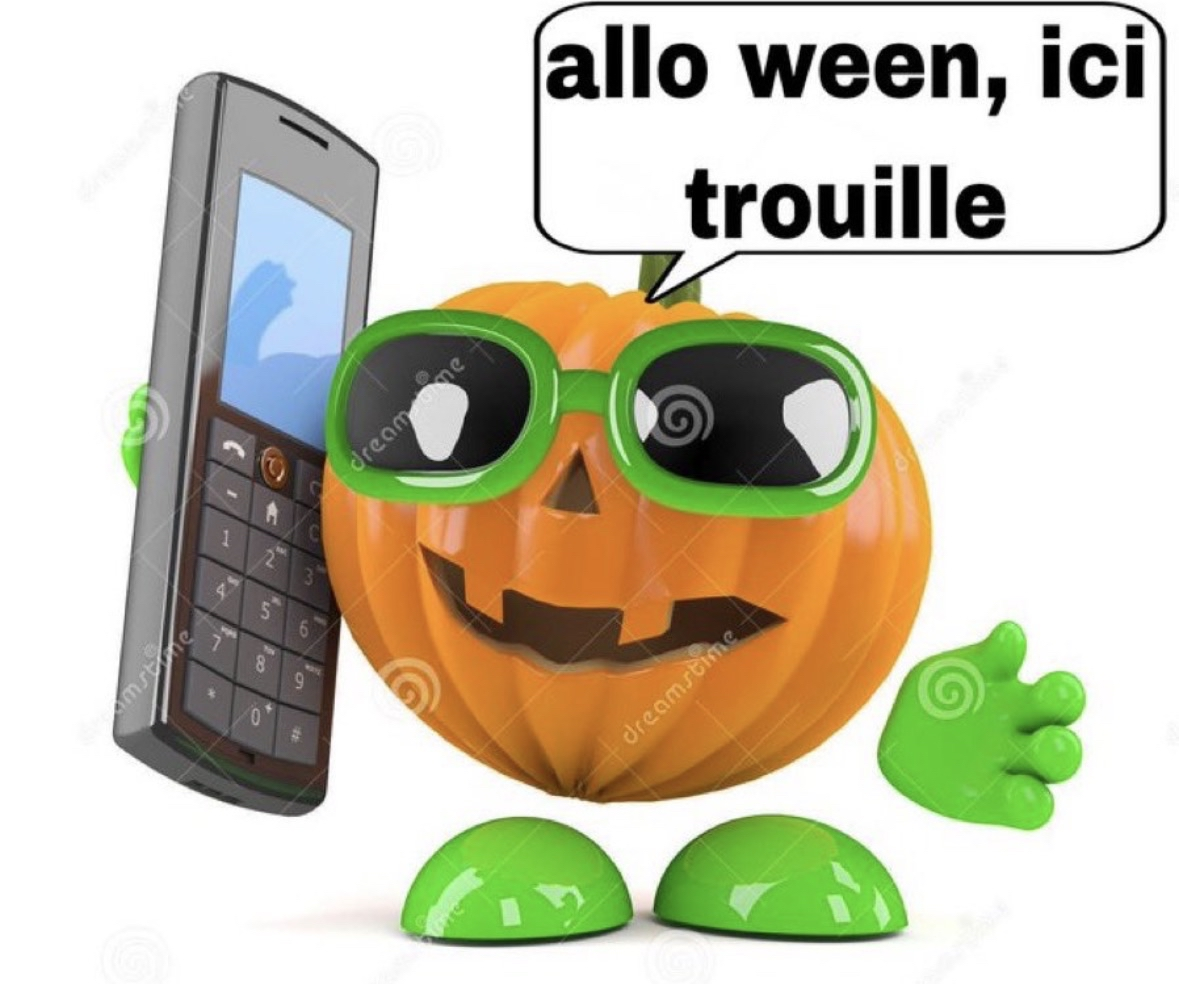
\includegraphics[width=160px]{./../autre/allo.png}
	\captionof{figure}{moi qui appelle ringot pr lui annoncer que le pendule coute 500€}
	
\end{document}
